% This is IJUC.TEX the demonstration file of
% the LaTeX macro package for International Journal of Unconventional Computation,
% version 0.1 for LaTeX2e

\documentclass{ijuc}
\usepackage[pdftex]{graphics}

\begin{document}

\title{IJUC formatting in \LaTeX}

\author{First Author\inst{1}\email{a1@ijuc.ac.uk}
\and A. N. Other Author\inst{2} 
\and Last Author\inst{3}
}

\institute{Department of Computer Science, University of IJUC, UK
\and
Department of Unconventional Computing, University of Elsewhere, USA
\and
Department of Biology, University of IJUC, UK
}

\def\received{Received 17 December 2004; In final form 1 April 2005}

\maketitle


\begin{abstract}
The title of the paper should clearly indicate the scope and findings
of the paper and should provide an accurate indication of the contents when
searched by computerized methods.
The abstract should be 100--150 words, summarizing the significant findings. 
\end{abstract}

\keywords{Six to twelve keywords or phrases, to aid in indexing the article.
}



\section{Introduction}

This describes the IJUC \LaTeX\ style
class file {\tt ijuc.cls} and the Bib\TeX\ file {\tt ijuc.bst},
suitable for processing with {\tt latex} or {\tt pdflatex}.
(This example file has a pdf figure example,
so should be processed with {\tt pdflatex}.)

\section{Formatting instructions}

\subsection{Figures and Tables}

Mention of figures and tables within text: When referring to figures, tables
and other elements within the text, always call the element by its full name (for
example: ``See Table 1,'' ``Figure 1 illustrates\ldots,'' ``Refer to Scheme 1.'' Do not
use ambiguous phraseologies (for example: ``1 illustrates\ldots'') that do not clearly
denote the element being referred to.


\subsubsection{Figures}

Tables are numbered consecutively and should include a clear
descriptive caption (see Figure \ref{fig-eg}).


\begin{figure}
\begin{center}
\scalebox{0.5}{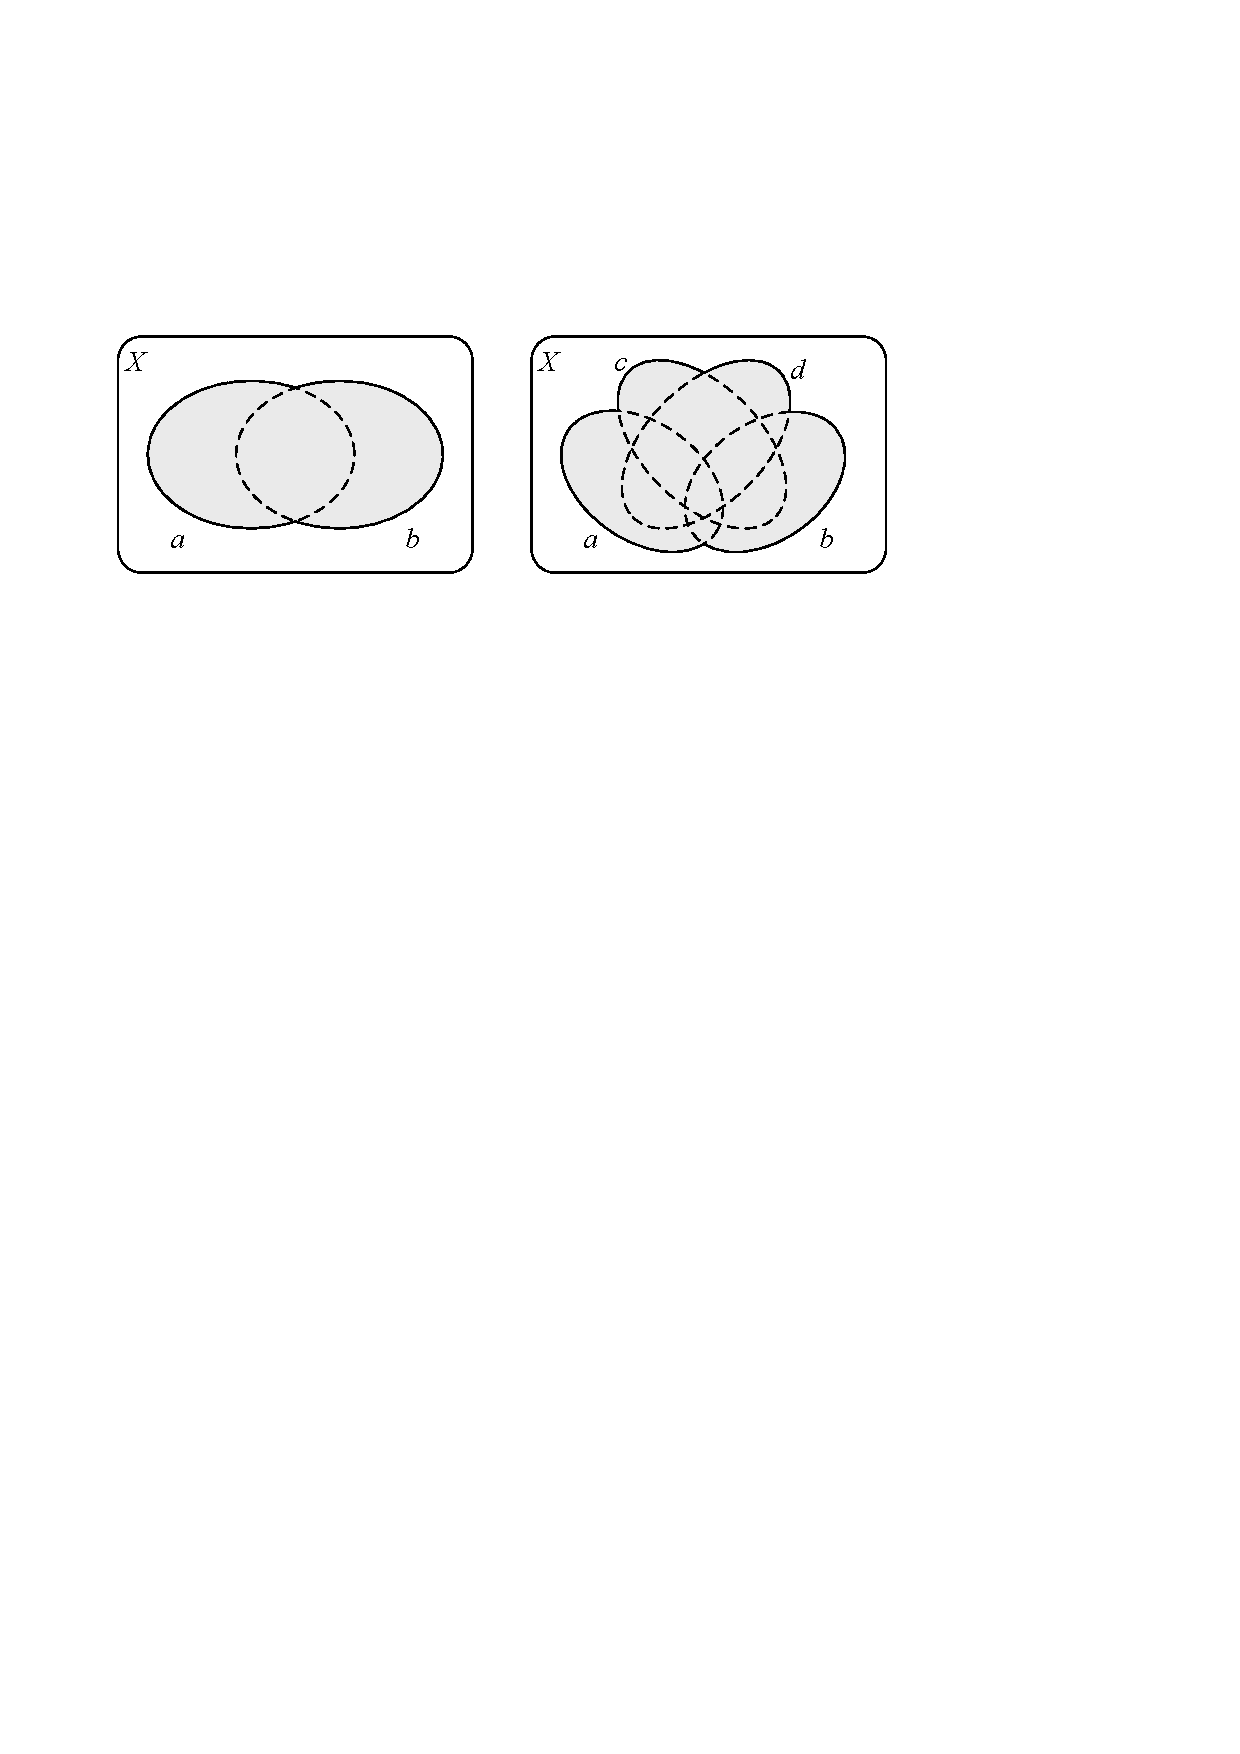
\includegraphics{union.pdf}}
\end{center}
\caption{Example figure, taken from reference \cite{St1}.}
\label{fig-eg}
\end{figure}




\subsubsection{Tables}

Tables are numbered consecutively and should include a clear
descriptive caption. Avoid the use of structural formulas in the body
of tables. Table footnotes should be given a footnote symbol as explained in
the Footnotes section, proceeding by row rather than by column order.
Footnotes within a table should be indicated by the same
symbols listed above. Reinitialize symbol sequence within tables. Place footnotes
to a table directly beneath the table. (See Table \ref{tbl-eg}).


\begin{table}
\begin{center}
\begin{tabular}{|@{\hspace{1mm}}c@{\hspace{1mm}}|c||c|c|@{\hspace{1mm}}c@{\hspace{1mm}}|}\hline
$X$ range&$R$ values&$\alpha$ \footnotemark[1] & $\mathit{MIL}$ \footnotemark[2]& $\mathit{MaxIL}$\\\hline
$-8$:20:2& 2.5, 3.0&0.97\footnotemark[3]&500&500\\\hline
$-8$:30:2&2.5&0.98&1000&1000\\\hline
\end{tabular}
\end{center}
\caption{Example table, excerpted from reference \cite{St2}.\\
{\footnotesize
\footnotemark[1]a footnote about $\alpha$;
\footnotemark[2]in row not column order;
\footnotemark[3]the last footnote
}
} 
\label{tbl-eg}
\end{table}



\subsection{Footnotes}

Authors are encouraged to minimize the use of footnotes. A
footnote may include the designation of a corresponding author of the paper,
current address information for an author (if different from that shown in the
affiliation), and traditional footnote content. 


Footnotes are indicated in the text by the following symbols:
asterisk\footnote{asterisk or star},
dagger\footnote{dagger}, 
double dagger\footnote{double dagger}, 
paragraph mark\footnote{paragraph mark}, 
section mark\footnote{section mark}, 
parallels\footnote{parallels}, 
number sign\footnote{number sign},
and then their doubled counterparts. 

Numerals are not used for footnote callouts,
as they may be mistaken for bibliographical reference call-outs or exponents.


\section{Acknowledgments}

Information concerning grant
support of research should appear in a separate Acknowledgments section at
the end of the paper, not in a footnote. Acknowledgments of the assistance of
colleagues or similar notes of appreciation also properly belong in an
Acknowledgments section, not in footnotes.


\section{Citing References}

References are indicated in the text by consecutive Arabic numbers
in brackets. The full list is collected at the end of the paper in numerical
order. All references in the list should be cited within the text, and vice
versa. Listed references should be complete in all details, including article
titles in journals. All authors on each paper should be cited; ``et al.'' is not sufficient.
Journal title abbreviations should conform to Mathematical Reviews
Index style.


\bibliography{ijuc}

\appendix 

\end{document}
